\documentclass[aspectratio=169]{beamer}

% select theme
\usetheme{CambridgeUS}
\usefonttheme{professionalfonts}
\usecolortheme{beaver}
\useinnertheme{rectangles}
\setbeamertemplate{theorems}[ams style] 

\usepackage{kotex}
\usepackage{fancyvrb}
\usepackage{color}
\usepackage{graphicx}
\usepackage[ruled,vlined]{algorithm2e}
\usepackage{hyperref}
\usepackage{minted}

% \newminted{python}{fontsize=\scriptsize, 
% 		   linenos,
% 		   numbersep=8pt,
% 		   gobble=4,
% 		   frame=lines,
% 		   bgcolor=bg,
% 		   framesep=3mm} 

% \usepackage{amsmath}

% \setfont


% \newcommand{\mathbb{E}}{\mathbb{E}}



\begin{document}

% \definecolor{bg}{rgb}{0.95,0.95,0.95}
% \defverbatim[colored]\toydata{
% \begin{pythoncode}
% 	p_y_x=np.exp(-(y-x)**2/(2*var))
% 	p_y_x_minus=np.exp(-(y+1)**2/(2*var))
% 	p_y_x_plus=np.exp(-(y-1)**2/(2*var))
% 	mi=np.average(np.log(p_y_x/(0.5*p_y_x_minus+0.5*p_y_x_plus)))
% 	mi # 0.6586568587377033
% \end{pythoncode}
% }


% title slide
\begin{frame}
	\title{MINE: Mutual Information Neural Estimation}
	\subtitle{ICML 2018}
	\author{Jaehyun Ko}
	\date{\today}
	\titlepage
\end{frame}


% outline slide
\section*{Outline}
\begin{frame}
\tableofcontents
\end{frame}



\section{Introduction}
\begin{frame}
	\frametitle{Introduction}
	\textbf{Motivation} \\ Estimate mutual information between two random variables using neural networks. \\
\end{frame}

% \begin{frame}
% 	\frametitle{Toy data}
% 	\textbf{Toy Data} \\ Two distribution
% 	\begin{align*}
% 		X &\sim \mathcal{N}(0,
% 		\begin{bmatrix}
% 			1 & 0 \\
% 			0 & 1
% 		\end{bmatrix})\\
% 		Y &\sim \mathcal{N}(0, 
% 		\begin{bmatrix}
% 			1 & 0.8 \\
% 			0.8 & 1
% 		\end{bmatrix})
% 	\end{align*}
% 	\begin{figure}
% 		\centering
% 		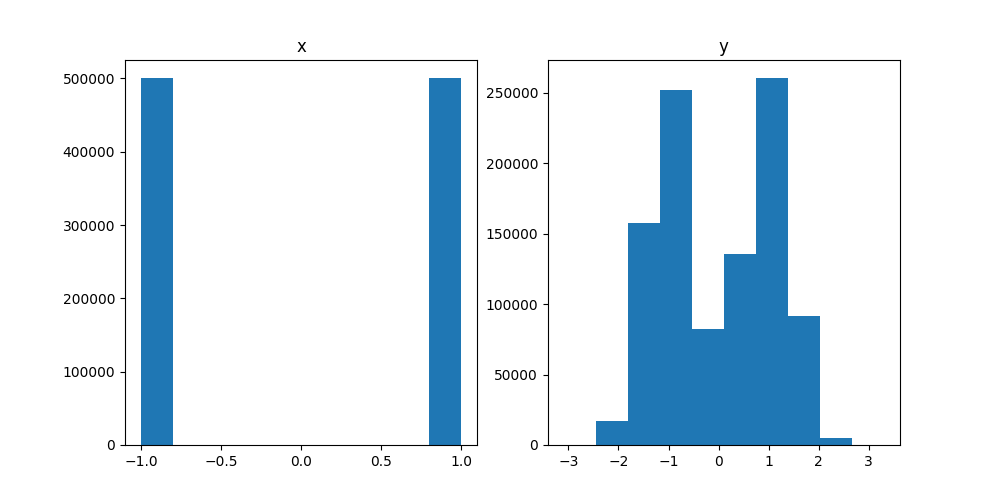
\includegraphics[width=0.3\textwidth]{./images/toy_data.png}
% 		\caption{Toy data}
% 		\label{fig:toy_data}
% 	\end{figure}
% \end{frame}



\section{Backgrounds}
\subsection{Information Theory}
\begin{frame}
	\frametitle{Entropy}
	\textbf{Entropy} is a measure of the uncertainty of a random variable.
	\begin{definition}
		\textbf{Entropy} For any probability density fuction p, entropy is defied as
		\begin{equation*}H(x) = \mathbb{E}_p [-\log p(x)] = - \int {p(x)\log{p(x)}dx}\end{equation*}
	\end{definition}
	\begin{itemize}
		\item \textbf{Entropy} is a measure of the uncertainty of a random variable.
		\item average bit-length to representate RV \cite{shannon1948mathematical}.
	\end{itemize}
\end{frame}

\begin{frame}
	\frametitle{Cross Entropy}
	The cross-entropy between two probability distributions $p$ and $q$
	over the same underlying set of events measures
	the average number of bits needed to identify an event
	drawn from the set if a coding scheme used for the set
	is optimized for an estimated probability distribution $q$, rather than the true distribution $p$.
	\begin{definition}
		\textbf{Cross Entropy}(CE) is defined as 
		\begin{equation*}H(p, q) = \mathbb{E}_p [-\log q(x)] = - \int p(x) \log q(x)dx\end{equation*}
	\end{definition}
	\end{frame}

\begin{frame}
	\frametitle{Kullback-Leibler Divergence}
	\begin{definition}
		\textbf{Kullback-Leibler Divergence} (KLD) For two probability densities p(x), q(x) is defined as
		\begin{equation*}D(p(x)||q(x))
			= \int p(x) \log \frac{p(x)}{q(x)}dx,\end{equation*}
	\end{definition}
	it can be interpreted as difference of two entropy.
	\begin{align*}
		D(p(x)||q(x)) = \int p(x) (-\log{q(x)})dx - \int p(x) (-\log{p(x)})dx \\
		= H(p, q) - H(p)
	\end{align*}
\end{frame}

\begin{frame}
	\frametitle{Mutual Information} 
	MI is a measure of the dependence between two random variables.
	\begin{definition} \label{def:mutual_information}
		\textbf{Mutual Information} (MI) Let $X$ and $Y$ be two random variables with a joint
		distribution $P(x, y)$ and $P_x$, $P_y$ are marginal probability distribution each.
		The Mutual Information $I(X;Y)$ is defined as
		\begin{equation*}I(X;Y) = \mathbb{E}_{P_{xy}} [\log\frac{P_{xy}}{P_x P_y}]\end{equation*}
	\end{definition}	
\end{frame}

\begin{frame}
	\frametitle{Mutual Information(cont.)}
	we can rewrite the mutual information as follows.
	\begin{align*}
		I(X;Z)&= \mathbb{E}_P[-\log P_x] - \mathbb{E}_P[-\log\frac{P_y}{P_{xy}}]\\
		&= H(X)-H(X|Z)
	\end{align*}
	MI between X and Z can be understood as the decrease of the uncertainty in X given Z.
	and it also representated as KLD between joint distribution and product of marginal distribution.
	\begin{equation}\label{eq:kl_form} I(X;Z) = D(P_{xy}||P_{x} \otimes P_{y}) \end{equation}
\end{frame}

\subsection{Donsker-Varadhan Variational Formula}
	\begin{frame}
		\frametitle{Donsker-Varadhan Representation}
		\begin{theorem}
			\textbf{Donsker-Varadhan Representation} (DV)
			Let $X$ be a random variable with domain $\mathcal{X}$, let P, Q be two probability density functions
			and $T$ be a function on $\mathcal{X}$, 
			Then, for any $x \in \mathcal{X}$, the KLD admits the following dual Representation
			\begin{equation*}
				D(P || Q) = \sup_{T:\mathcal{X} \rightarrow \mathbb{R}} \{ \mathbb{E}_P[T] - \log \mathbb{E}_Q[e^{T}]\}
			\end{equation*}
		\end{theorem}
		the proof of theorem consists of two steps.
		\begin{itemize}
			\item \textbf{Step 1} : Existence of supremum in Donsker-Varadhan variational representation
			\item \textbf{Step 2} : Lower bound for the Kullback Liebler Divergence
		\end{itemize}	
	\end{frame}

	\begin{frame}
		\frametitle{Donsker-Varadhan Representation(cont.)}
		\framesubtitle{Existence of supremum in Donsker-Varadhan variational representation}
		\begin{lemma}
			There exists a function $T^*: X \rightarrow \mathbb{R}$ such that satisfies the condition of equality.
		\end{lemma}
		choise $T^* = \log\frac{P}{Q}$, then prove in the following page.
	\end{frame}


	\begin{frame}
		\frametitle{Donsker-Varadhan Representation(cont.)}
		\framesubtitle{Existence of supremum in Donsker-Varadhan variational representation}
		\begin{align}
			D_{\text{KL}}(P|Q) &= \mathbb{E}_P[T^*(X)] - \log(\mathbb{E}_Q[e^{T^*(X)}])\\			
			% \mathbb{E}_P[T(X)] - \log(\mathbb{E}_Q[e^{T(X)}])
			&= \mathbb{E}_P [\log \frac{P(X)}{Q(X)}]-\log(\mathbb{E}_Q[e^{\log\frac{P(X)}{Q(X)}}])\\
			&= D_{\text{KL}}(P|Q) - \log(\mathbb{E}_Q[\frac{P(X)}{Q(X)}])\\
			&= D_{\text{KL}}(P|Q) - \log(\int_{\mathcal{X}} Q(x)\frac{P(x)}{Q(x)}dx)\\
			&= D_{\text{KL}}(P|Q) - \log(\int_{\mathcal{X}} P(x)dx)\\
			&= D_{\text{KL}}(P|Q) - \log(1)\\
			&= D_{\text{KL}}(P|Q)
		\end{align}
	\end{frame}

	\begin{frame}
		\frametitle{Donsker-Varadhan Representation(cont.)}
		\framesubtitle{Lower bound for the Kullback Liebler Divergence}
		\begin{lemma}\label{lemma:lower_bound}
			For any function $T:X \rightarrow \mathbb{R}$ the following inequality holds:
			$D_{\text{KL}}(P | Q) \geq \sup_{T: \mathcal{X} \rightarrow \mathbb{R}} {\mathbb{E}_P[T(X)] - \log \mathbb{E}_Q[e^{T(X)}]}$
		\end{lemma}
		suppose new probability density function $G$ is defined as follows:
		\begin{align}
			G(x) &=\frac{Q(x)e^T}{\mathbb{E}_Q[e^{T(X)}]}\\
			\int_{\mathcal{X}} G(x)dx = \frac{\int_{\mathcal{X}} Q(x)e^T}{\mathbb{E}_Q[e^{T(X)}]} 
			&=\frac{\mathbb{E}_Q[e^{T(X)}]}{\mathbb{E}_Q[e^{T(X)}]} = 1 
		\end{align}
	\end{frame}

	\begin{frame}
		\frametitle{Donsker-Varadhan Representation(cont.)}
		\framesubtitle{Lower bound for the Kullback Liebler Divergence}
		\begin{align}
			&D_{\text{KL}}(P | Q) -\sup_{T: \mathcal{X} \rightarrow \mathbb{R}} {\mathbb{E}_P[T(X)] + \log \mathbb{E}_Q[e^{T(X)}]}\\
			&= \mathbb{E}_P[\log \frac{P(X)}{Q(X)}-T(X)] + \log(\mathbb{E}_Q[e^{T(X)}])\\
			&= \mathbb{E}_P[\log \frac{P(X)}{Q(X) e^{T(X)}}] - \log(\mathbb{E}_Q[e^{T(X)}])\\
			&= \mathbb{E}_P[\log \frac{P(X)\mathbb{E}_Q[e^{T(X)}]}{Q(X) e^{T(X)}}]\\
			&= \mathbb{E}_P[\log \frac{P(X)}{G(X)}]\\
			&= D_{\text{KL}}(P|G) \geq 0
		\end{align}
	\end{frame}
	% \begin{align*}

	% \end{align*} 
	
	% \begin{equation*}

	% \end{equation*}

% \end{frame}

\section{MINE}
\begin{frame}
	\frametitle{MINE}
	\framesubtitle{Mutual Information Neural Estimation}
	in this section, we will Donsker-Varadhan variational formulation in order to estimate mutual information,
	via approximating $T$ using neural network. according to discussion so,
	we can estimate the mutual information by maximizing the following cost function:
	% \autoref{eq:kl_form} 
	\begin{equation}\label{eq:mine}
		I(X;Y) = \sup_{T: \mathcal{X} \times \mathcal{Y} \rightarrow \mathbb{R}}
		{\mathbb{E}_{P_{XY}}[T(X,Y)] - \log \mathbb{E}_{P_X \otimes P_Y}[e^{T(X,Y)}]}
	\end{equation}
\end{frame}

\begin{frame}
	\frametitle{MINE(cont.)}
	\framesubtitle{Estimation of each term of MINE}
	In order to estimate each term of MINE (\autoref{eq:mine}),
	\begin{enumerate}
		\item we need to the full knowlage of the joint and marginal distribution of $X$ and $Y$.
		\item we need to find maximization of $T(X,Y)$ over all possible functions, $T \in \mathcal{F}$.
	\end{enumerate}
\end{frame}

\begin{frame}
	\frametitle{MINE(cont.)}
	\framesubtitle{Estimation of each term of MINE}
	In assume that we have a sample of $n$ independent and identically distributed samples from $P_{XY}$. \\
	then, we can use the law of large numbers to obtain following approximation of the first expectation:
	\begin{equation} \label{eq:mine_first_term}
		\mathbb{E}_{P_{XY}}[T(X,Y)] \approx \frac{1}{n} \sum_{i=1}^n T(X_i, Y_i)
	\end{equation}	
\end{frame}

\begin{frame}
	\frametitle{MINE(cont.)}
	\framesubtitle{Estimation of each term of MINE}
	To obtain an approximation of the second expectation, we cannot use the law of large numbers,
	because the expectation is over the product of two random variables.\\
	We can use some tricks: suffling. artificially construct a tuple set $(X_i, \tilde{Y_i})$,
	where $\tilde{Y_i}$ is a randomly sampled from $(Y_i)^n_{i=1}$.\\
	Then, we can use the law of large numbers to obtain following approximation of the second expectation:
	\begin{equation}\label{eq:mine_second_term}
		\mathbb{E}_{P_X \otimes P_Y}[e^{T(X,Y)}] \approx \frac{1}{n} \sum_{i=1}^n T(X_i, \tilde{Y_i})
	\end{equation}	
\end{frame}

\begin{frame}
	\frametitle{MINE(cont.)}
	\framesubtitle{Estimation of each term of MINE}
	Now, we can estimate the mutual information by maximizing the following cost function:
	\begin{equation}\label{eq:mine_cost}
		\hat{I}(X;Y) = \sup_{T: \mathcal{X} \times \mathcal{Y} \rightarrow \mathbb{R}}
			{\frac{1}{n} \sum_{i=1}^n T(X_i, Y_i) - \log \frac{1}{n} \sum_{i=1}^n T(X_i, \tilde{Y_i})}
	\end{equation}
\end{frame}

\begin{frame}
	\begin{center}
		\begin{minipage}{0.8\linewidth}
			% \setframetitle{MINE Algorithm}
			\begin{algorithm}[H]
				\DontPrintSemicolon
				\SetAlgoLined
				\KwIn{Joint distribution $P_{XY}$ and neural network architecture}
				\KwOut{An estimate of the mutual information $I(X;Y)$}
				Initialize network parameters $\theta$\
				\Repeat{convergence}{
				Draw mini-batch of samples: $(X_1, Y_1), (X_2, Y_2), \ldots, (X_n, Y_n) \sim P_{XY}$\;
				Draw $n$ samples from the marginal distribution: $\tilde{Y_{1}}, \tilde{Y_{2}}, \ldots, \tilde{Y_{n}} \sim P_Y$\;
				Evaluate: $\hat{I}_\theta(X; Y) \rightarrow \frac{1}{n} \sum_{i=1}^n T_\theta(X_i, Y_i) - \log(\frac{1}{n}\sum_{i=1}^n e^{T_\theta(X_i, \tilde{Y_i})})$\;
				Update network parameters: $\theta \rightarrow \theta + \nabla_\theta \hat{I}_\theta(X; Y)$\;
				}
				\Return An estimate of the mutual information $I_{\theta}(X;Y)$\
				\caption{Mutual Information Neural Estimation (MINE)}
				\label{alg:mine}
			\end{algorithm}
		\end{minipage}
	\end{center}
\end{frame}

\section{Theoretical Properties}
\begin{frame}
	\frametitle{Strong Consistency}
	\framesubtitle{Proof of Approxiation of MINE}
	\begin{definition}
		\label{def:strong_consistency}
		The estimater $\hat{I}_\theta(X;Y)$ is said to be strongly consistent if: \\
		for all $\epsilon > 0$, there exists a positive integer $N$ and a choice of statistics network such that: \\
		\begin{equation}
			\forall n \geq N, | I(X;Y) - \widehat{I_\theta(X;Y)}_n | \leq \epsilon
		\end{equation}
		where the probability is over a set of samples.
	\end{definition}
\end{frame}

\section{Experiments}
\begin{frame}
	\frametitle{Toy data}
	Two distribution
	\begin{align*}
		X &\sim \text{sgn}(\mathcal{N}(0,1)) \\
		Y &\sim X+\mathcal{N}(0, 0.2)
	\end{align*}
	\begin{figure}
		\centering
		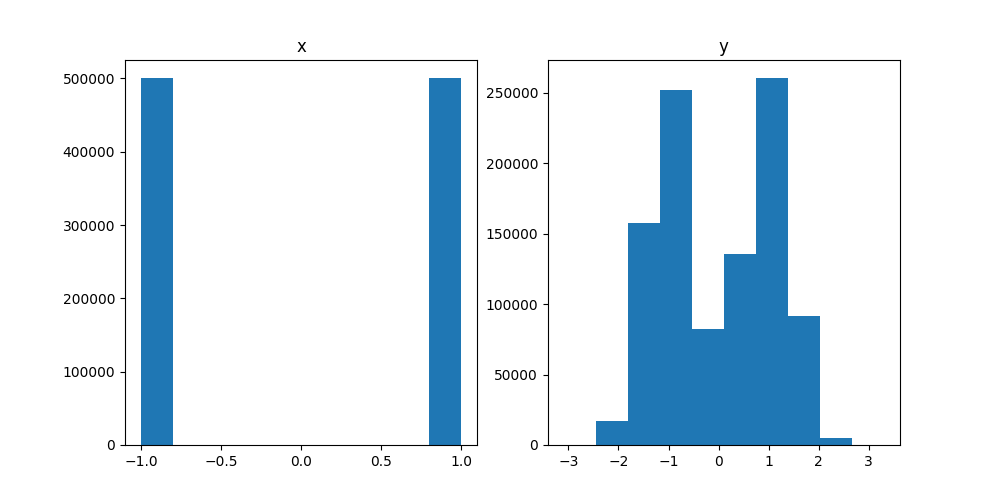
\includegraphics[width=0.5\textwidth]{./images/toy_data.png}
		\caption{Toy data}
		\label{fig:toy_data}
	\end{figure}
\end{frame}

\begin{frame}
	\frametitle{Toy data}
	compute mutual information of two distribution directly
	\begin{align*}
		I(X;Y)	&\approx \frac{1}{n} \sum_{i=1}^n \frac{\log{P_{X,Y}(x_i, y_i)}}{\log{P_X(x_i)}{P_Y(y_i)}} \\
		& = \frac{1}{n} \sum_{i=1}^n \log{\frac{{P_{Y|X}(y_i|x_i)}}{{P_{Y|X}(y_i|X)}{P_X(X)}}} \\
		& = \frac{1}{n} \sum_{i=1}^n \log{\frac{{P_{Y|X}(y_i|x_i)}}{{0.5 P_{Y|X}(y_i|X = -1)} + {0.5 P_{Y|X}(y_i|X = 1)}}}
	\end{align*}
\end{frame}

\begin{frame}
	\toydata
\end{frame}

% \section{Application}

% \section{Conclusion}

\section{Refrences}
\begin{frame}
	\bibliographystyle{plain} % We choose the "plain" reference style
	\bibliography{ref.bib} % Entries are in the refs.bib file
	% \printbibliography 
\end{frame}

\end{document}

